\documentclass[11pt,oneside,letterpaper]{article}

% graphicx package, useful for including eps and pdf graphics
\usepackage{graphicx}
\DeclareGraphicsExtensions{.pdf,.png,.jpg}

% basic packages
\usepackage{color} 
\usepackage{parskip}
\usepackage{float}

% text layout
\usepackage{geometry}
\geometry{textwidth=15cm} % 15.25cm for single-space, 16.25cm for double-space
\geometry{textheight=22cm} % 22cm for single-space, 22.5cm for double-space

% helps to keep figures from being orphaned on a page by themselves
\renewcommand{\topfraction}{0.85}
\renewcommand{\textfraction}{0.1}

% bold the 'Figure #' in the caption and separate it with a period
% Captions will be left justified
\usepackage[labelfont=bf,labelsep=period,font=small]{caption}

% review layout with double-spacing
%\usepackage{setspace} 
%\doublespacing
%\captionsetup{labelfont=bf,labelsep=period,font=doublespacing}

% cite package, to clean up citations in the main text. Do not remove.
\usepackage{cite}
%\renewcommand\citeleft{(}
%\renewcommand\citeright{)}
%\renewcommand\citeform[1]{\textsl{#1}}

% Remove brackets from numbering in list of References
\renewcommand\refname{\large References}
\makeatletter
\renewcommand{\@biblabel}[1]{\quad#1.}
\makeatother

\usepackage{authblk}
\renewcommand\Authands{ \& }
\renewcommand\Authfont{\normalsize \bf}
\renewcommand\Affilfont{\small \normalfont}
\makeatletter
\renewcommand\AB@affilsepx{, \protect\Affilfont}
\makeatother

% notation
\usepackage{amsmath}
\usepackage{amssymb}
\newcommand{\normal}{\mathcal{N}}					% Normal distribution
\setlength{\arraycolsep}{2pt}
\newcommand{\twomatrix}[2]{\left( \begin{matrix} #1 \\ #2 \end{matrix} \right)}								% pretty inline matrix 
\newcommand{\fourmatrix}[4]{\left( \begin{matrix} #1 & #2 \\ #3 & #4 \end{matrix} \right)}					% pretty inline matrix 

\setcounter{figure}{2}
\setcounter{table}{0}
\setcounter{page}{1}
\renewcommand{\thefigure}{S\arabic{figure}}
\renewcommand{\thetable}{S\arabic{table}}
\renewcommand{\thepage}{S\arabic{page}}

%%% TITLE %%%
\title{\vspace{1.0cm} \LARGE \bf 
Supporting Text: \\
Integrating influenza antigenic dynamics with molecular evolution
}

\author[1]{Trevor Bedford}
\author[2,3,4]{Marc A. Suchard}
\author[5]{Philippe Lemey}
\author[1]{Gytis Dudas}
\author[6]{Victoria Gregory}
\author[6]{Alan J. Hay}
\author[6]{John W. McCauley}
\author[7]{Colin A. Russell}
\author[7,8]{Derek J. Smith}
\author[1,9]{Andrew Rambaut}

\affil[1]{Institute of Evolutionary Biology, University of Edinburgh, Edinburgh, UK}
\affil[2]{Department of Biomathematics, David Geffen School of Medicine at UCLA, University of California, Los Angeles CA, USA}
\affil[3]{Department of Human Genetics, David Geffen School of Medicine at UCLA, University of California, Los Angeles CA, USA}
\affil[4]{Department of Biostatistics, UCLA Fielding School of Public Health, University of California, Los Angeles CA, USA}
\affil[5]{Department of Microbiology and Immunology, Katholieke Universiteit Leuven, Leuven, Belgium}
\affil[6]{Division of Virology, MRC National Institute for Medical Research, Mill Hill, London, UK}
\affil[7]{Department of Zoology, University of Cambridge, Cambridge, UK.}
\affil[8]{Department of Virology, Erasmus Medical Centre, Rotterdam, Netherlands.}
\affil[9]{Fogarty International Center, National Institutes of Health, Bethesda, MD, USA.}

\date{}

\begin{document}

\maketitle

%%% SUPPORTING METHODS %%%
\section*{Supporting Methods}

\subsection*{Genetic, antigenic and surveillance data}

We compiled an antigenic dataset of hemagglutination inhibition (HI) measurements of virus isolates against post-infection ferret sera for influenza A/H3N2 by collecting data from previous publications \cite{Hay01,Smith04,Russell08,Barr10}, NIMR vaccine strain selection reports for 2002 and 2008--2012 \cite{NIMR02,NIMRMarch08,NIMRFeb09,NIMRFeb10,NIMRSep10,NIMRSep11,NIMRFeb12} and the Feb 2011 VRBPAC report \cite{Cox11FDA}.
We queried the Influenza Research Database \cite{IRD} and the EpiFlu Database \cite{GISAID} for HA nucleotide sequences by matching strain names, e.g.\ A/HongKong/1/1968, and only strains for which sequence was present was retained.
If a strain had multiple sequences in the databases we preferentially kept the IRD sequence and preferentially kept the longest sequence in IRD. 
Sequences were aligned using MUSCLE v3.7 under default parameters \cite{MUSCLE}.
This dataset had 2051 influenza isolates (present as either virus or serum in HI comparisons) dating from 1968 to 2011. 
However, the majority of isolates were present from 2002 to 2007. 
Because we are interested in longer-term antigenic evolution, we subsampled the data to have at most 20 virus isolates per year, preferentially keeping those isolates with more antigenic comparisons. 
We then kept only those serum isolates that are relatively informative to the antigenic placement of viruses, dropping serum isolates that are compared to 4 or fewer different virus isolates.
This censoring left 402 virus isolates, 519 serum isolates and 10,059 HI measurements. 
Each virus isolate was compared to an average of 21.9 serum isolates, and each serum isolate was compared to an average of 18.0 virus isolates.

Antigenic data for influenza A/H1N1 was collected from previous publications \cite{Kendal78,Webster79,Nakajima79,Nakajima81,Chakraverty82,Pereira82,Chakraverty86,Cox83,Daniels85,Raymond86,Stevens87,Donatelli93,Hay01,Daum02,McDonald07,Barr10} and NIMR vaccine strain selection reports for 2002--2010 \cite{NIMR02,NIMR03,NIMR04,NIMRFeb05,NIMRSep05,NIMRMarch06,NIMRSep06,NIMRMarch07,NIMRSep07,NIMRMarch08,NIMRSep08,NIMRFeb09,NIMRFeb10}.
The same procedure was followed as was followed for H3N2 to match sequence data and to subsample antigenic comparisons.
This procedure yielded 115 virus isolates, 77 serum isolates and 1882 HI measurements over the course of 1977 to 2009.
Each virus isolate was compared to an average of 10.0 serum isolates, and each serum isolate was compared to an average of 16.2 virus isolates.

Antigenic comparisons for influenza B/Victoria were collated from previous publications \cite{Rota90, Hay01, Muyanga01, Shaw02, Ansaldi04, Puzelli04, Xu04, Barr06, Daum06, Lin07} and vaccine strain selection reports for 2002--2012 \cite{AusWHO06, NIMR02, NIMR03, NIMR04, NIMRFeb05, NIMRSep05, NIMRMarch06, NIMRSep06, NIMRMarch07, NIMRSep07, NIMRMarch08, NIMRFeb09, NIMRSep09, NIMRFeb10, NIMRSep10, NIMRFeb11, NIMRSep11, NIMRFeb12}.
Here, the sequence matching and subsampling procedure yielded 179 virus isolates, 70 serum isolates and 2003 HI measurements over the course of 1986 to 2011.
Each virus isolate was compared to an average of 6.5 serum isolates, and each serum isolate was compared to an average of 16.7 virus isolates.

Antigenic comparisons for influenza B/Yamagata were collected from previous publications \cite{Rota90, Kanegae90, Nakajima92, Nerome98, Hay01, Muyanga01, Nakagawa02, Abed03, Ansaldi03, Ansaldi04, Matsuzaki04, Puzelli04, Shaw02, Xu04, Barr06, Daum06, Lin07} and vaccine strain selection reports for 2002--2012 \cite{AusWHO06, NIMR02, NIMR03, NIMR04, NIMRFeb05, NIMRSep05, NIMRMarch06, NIMRSep06, NIMRMarch07, NIMRSep07, NIMRMarch08, NIMRFeb09, NIMRSep09, NIMRFeb10, NIMRSep10, NIMRFeb11, NIMRSep11, NIMRFeb12}.
For B/Yamagata, the matching and subsampling procedure resulted in 174 virus isolates, 69 serum isolates and 1962 HI measurements over the course of 1987 to 2011.
Each virus isolate was compared to an average of 6.9 serum isolates, and each serum isolate was compared to an average of 17.3 virus isolates.

Surveillance data was obtained from the Centers of Disease Control and Prevention FluView Influenza Reports from the yearly summaries of influenza seasons 1997--1998 to 2010--2011 \cite{CDCReports}.
As an example, one report states ``collaborating laboratories in the United States tested 195,744 respiratory specimens for influenza viruses, 27,682 (14\%) of which were positive. Of these, 18,175 (66\%) were positive for influenza A viruses, and 9,507 (34\%) were positive for influenza B viruses. Of the 18,175 specimens positive for influenza A viruses, 7,631 (42\%) were subtyped; 6,762 (87\%) of these were seasonal influenza A (H1N1) viruses, and 869 (13\%) were influenza A (H3N2) viruses.''
In this case, we estimate the relative proportion of A/H3N2 of the four clades as $0.66 \times 0.13 = 0.09$.
Similar calculations were performed for A/H1N1, B/Vic and B/Yam.

\subsection*{Estimation of diffusion coefficient}

The distance $d$ traveled by a diffusion is not a linear function of time interval $t$, and thus the `rate' of diffusion cannot be calculated following $r=d/t$.
Assume we have a one-dimensional diffusion starting from $x_0 = 0$, so that
\begin{equation}
	X_t \sim \normal(0, \sigma^2 t),
\end{equation}
where $\sigma$ represents the diffusion volatility, and in this case, the expected squared displacement follows
\begin{equation}
	\mathrm{E}[X_t^2] = \sigma^2 t.
\end{equation}
In moving to a two-dimensional diffusion
\begin{equation}
	(X_t, Y_t) \sim \normal \left( \twomatrix{0}{0}, \fourmatrix{\sigma_x^2 t}{\rho \sigma_x \sigma_y t}{\rho \sigma_x \sigma_y t}{\sigma_y^2 t} \right),
\end{equation}
where $\sigma_x$ represents volatility in dimension 1, $\sigma_y$ represents volatility in dimension 2 and $\rho$ represents correlation,   expected squared displacement is equal to the sum of squared displacements in each dimension
\begin{equation}
	\mathrm{E}[X_t^2 + Y_t^2] = \sigma_x^2 t + \sigma_y^2 t.
\end{equation}
Such diffusions are often characterized with diffusion coefficient $D$.
In this case
\begin{equation}
	D = \frac{\sigma_x^2 + \sigma_y^2}{4},
\end{equation}
so that expected squared displacement follows from $D$ alone
\begin{equation}
	\mathrm{E}[X_t^2 + Y_t^2] = 4 D t.
\end{equation}

Owing to this relationship, Pybus et al.\ \cite{Pybus12} estimate $D$ from phylogenies in which internal nodes have inferred 2D locations via the formula
\begin{equation} \label{pybusest}
	\hat{D} = \frac{1}{n} \sum^n_{i=1} \frac{d_i^2}{4t_i},
\end{equation}
in which $d_i$ represents the displacement of a branch and $t_i$ represents the length of a branch.
However, uncertainty in $d_i$ or $t_i$, especially along short branches of the phylogeny, may cause $d_i^2/4t_i$ to have high variance and increase uncertainty in the resulting estimates of $D$.
Consequently, we estimate $D$ by looking at the relationship between total squared displacement and total time along branches of a phylogeny
\begin{eqnarray} \label{ourest}
	d^2_\Sigma &=& \sum^n_{i=1} d^2_i \nonumber \\
	t_\Sigma &=& \sum^n_{i=1} t_i \nonumber \\
	\hat{D} &=& \frac{ d^2_\Sigma }{ 4 t_\Sigma }.
\end{eqnarray}
This estimator showed less variance than equation \ref{pybusest} when analyzing tree output from the BMDS model and was thus preferred.
Additionally, we confirmed through simple simulation that estimator \ref{ourest} shows lower mean squared error than estimator \ref{pybusest} in the presence of modest levels of noise on estimates of $d_i$ and $t_i$.
When estimating $D$ specific to trunk branches or specific to side branches, we calculate $d^2_\Sigma$ and $t_\Sigma$ only from a subset of phylogeny branches as appropriate.

%%% SUPPORTING DISCUSSION %%%
\section*{Supporting Discussion}

\subsection*{Comparison with previous results}

Here, we attempt to compare antigenic locations inferred by our BMDS model to antigenic locations previously inferred by the error minimization methods of Smith et al.\ \cite{Smith04}, referred to here as antigenic cartography by MDS.
For this comparison, we use exactly the same HI data used to produce the results in \cite{Smith04}, consisting of 273 virus isolates, 79 serum isolates and a total of 4252 HI measurements taken between 1968 and 2003.
We begin with a BMDS analog of the antigenic model used in \cite{Smith04}, where serum effects are taken as the maximum titer of a particular ferret serum and the expected log$_2$ drop in HI titer is proportional to Euclidean distance between virus and serum locations.
To bring models into further alignment, we use a Uniform$(-100,100)$ distribution over virus locations and serum locations.
Unsurprisingly, we find that this BMDS model produces results that are strongly congruent with MDS results (Figure~\ref{smith_comparison}).
Antigenic cluster locations are consistent between methods (Figure~\ref{smith_comparison}A--B) and antigenic distances between pairs of viruses are consistent between temporally similar and temporally divergent viruses (Figure~\ref{smith_comparison}C--E), suggesting that the resulting maps are consistent at both local and global scales.
Credible intervals of antegenic distances for the BMDS model remain narrow across the temporal spectrum (Figure~\ref{smith_comparison}C--E), implying a fair degree of rigidity to the map.

%%% smith_comparison %%%
\begin{figure}[H]
	\centering		
	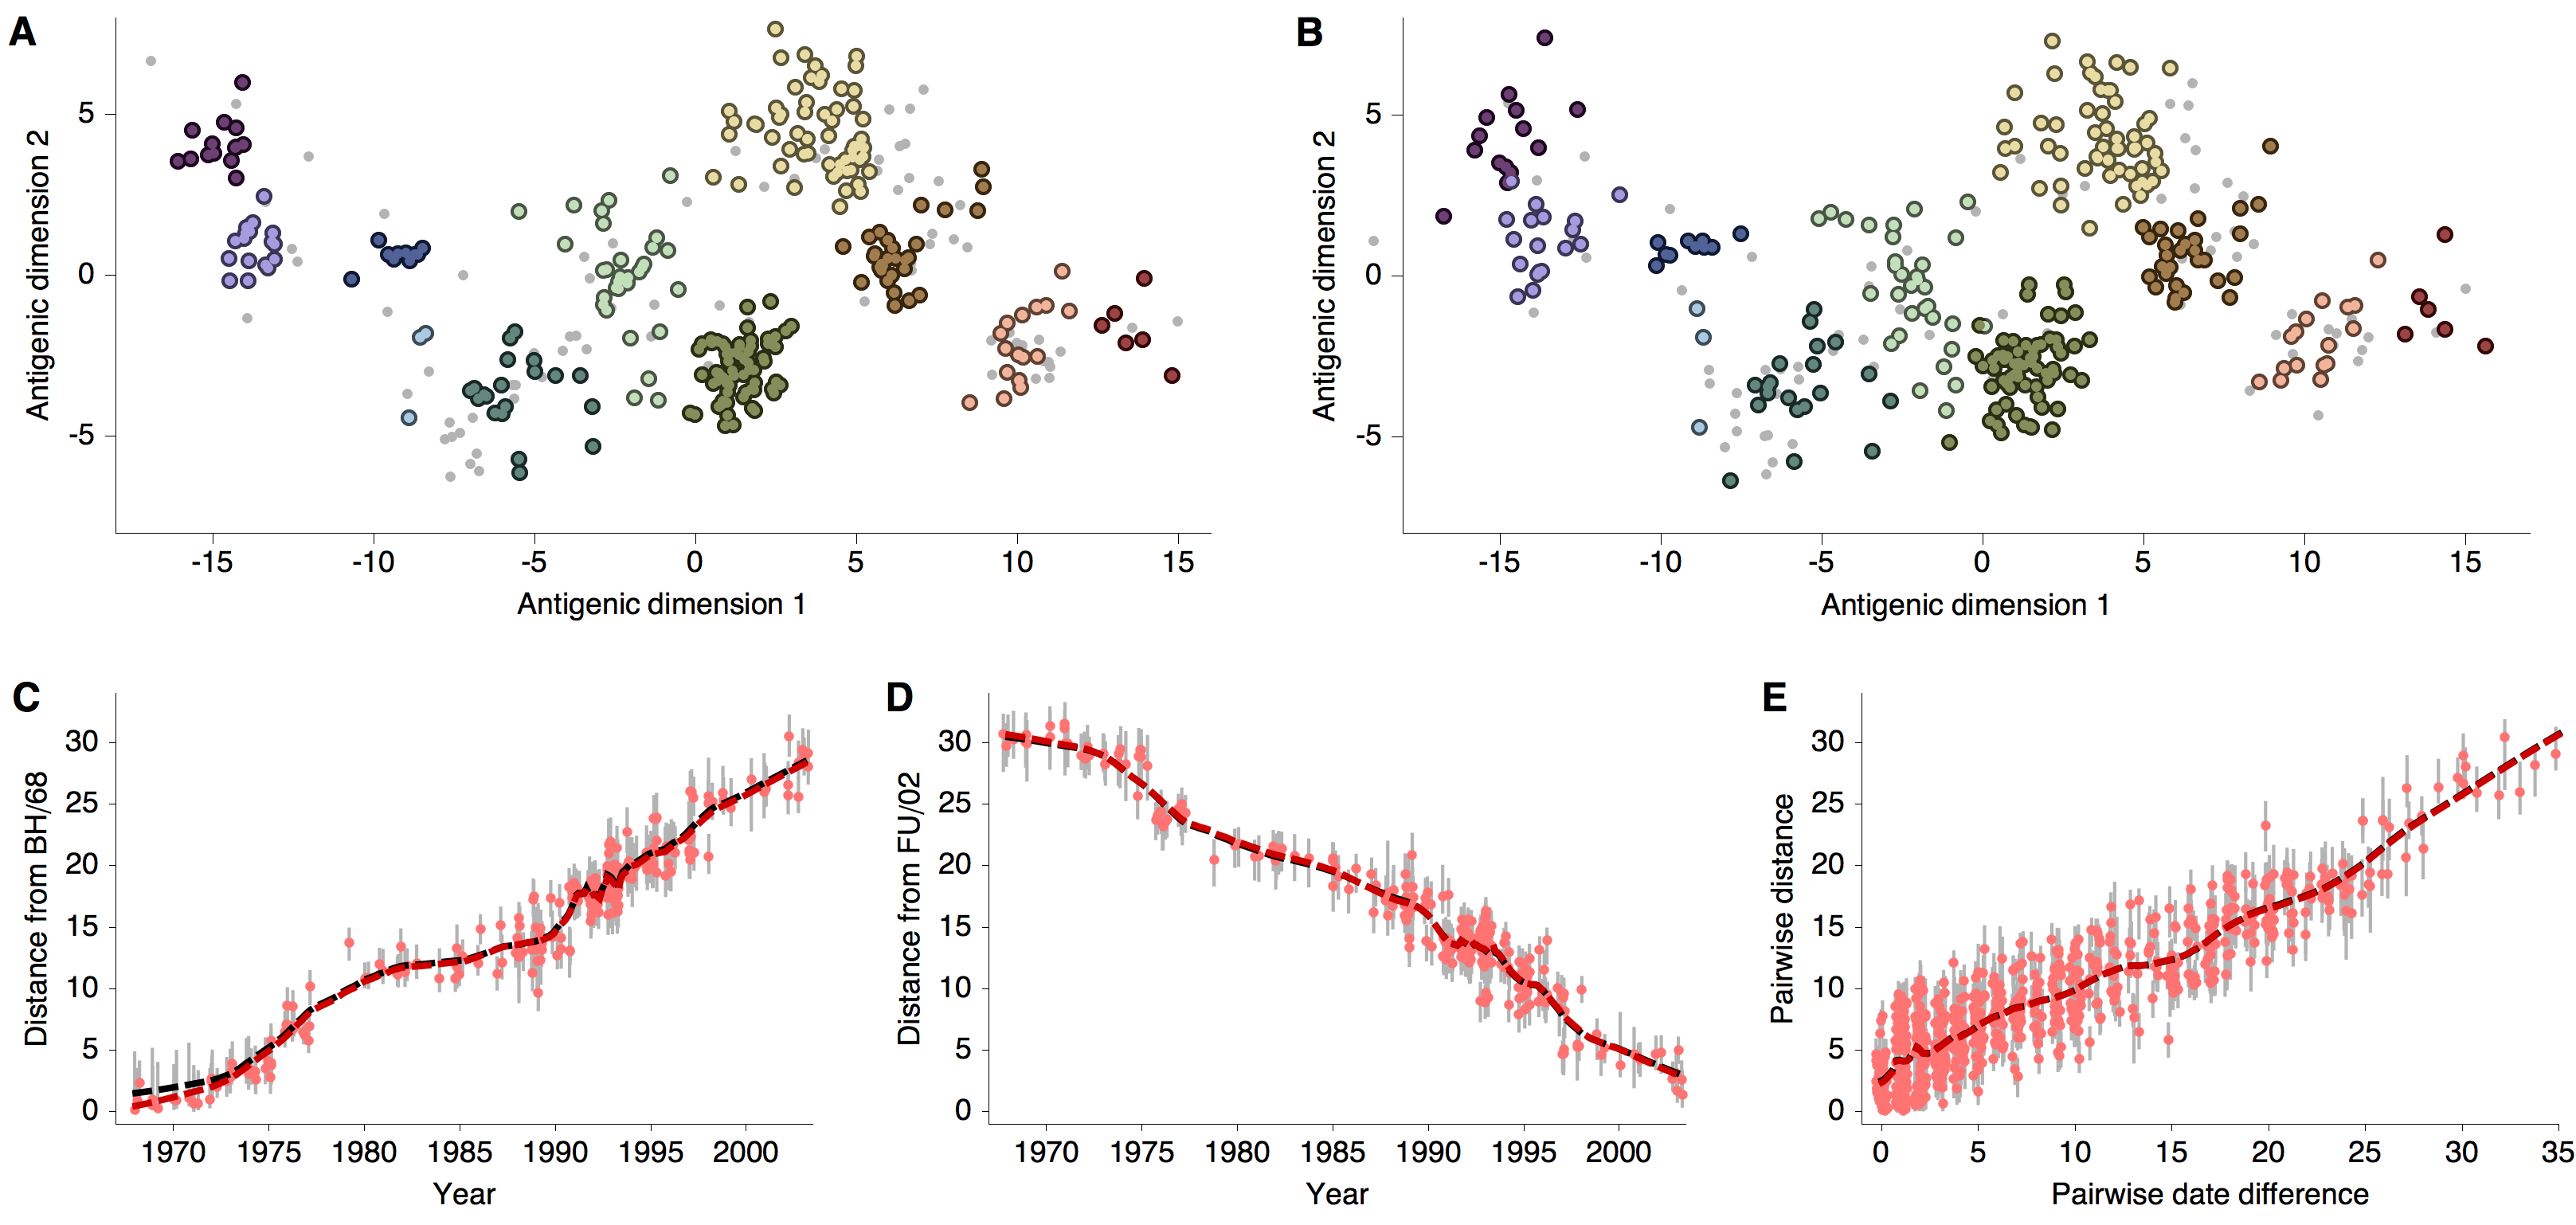
\includegraphics[width=1.0\textwidth]{figures/smith_comparison}
	\caption{\textbf{Comparison of A/H3N2 antigenic locations estimated by Smith et al.\ \cite{Smith04} using MDS and an equivalent BMDS model.} 
	(A) MDS antigenic locations, reorientated so that the primary dimension lies on the $x$-axis rather than on the $y$-axis as in Figure 1 of \cite{Smith04}.
	(B) A posterior sample of antigenic locations from an equivalent BMDS model.
	In (A) and (B), viruses are shown as colored circles, with color denoting antigenic cluster inferred by \cite{Smith04}, and sera are shown as gray points.
	(C) Antigenic distances between A/Bilthoven/16190/1968 and all other viruses determined for both methods.
	(D) Antigenic distances between A/Fujian/411/2002 and all other viruses determined for both methods.
	(E) Antigenic distances between 750 random pairs of viruses determined for both methods.	
	In (C), (D) and (E) red points show distances for the MDS model and gray bars show the 95\% credible interval of distances for the BMDS model, while the red dashed line shows a LOESS regression to MDS distances, and the black dashed line shows a LOESS regression to the BMDS distances.
	The BMDS model has a Uniform$(-100,100)$ prior on antigenic locations and serum effects fixed at maximum titer values. 
	} 
	\label{smith_comparison} 
\end{figure}

Smith et al.\ \cite{Smith04} show that there exist at least two solutions in their assignment of antigenic locations, involving the rotation of clusters HK/68, EN/72 and VI/75 (shown in Figure S2 of \cite{Smith04}).
We observe the same metastable behavior in our analysis; some MCMC chains converge on the solution shown in Figure \ref{smith_comparison}B, while other MCMC chains converge on the alternative solution shown in Figure \ref{smith_comparison_rotation}B.
The distribution of likelihood values appear highly similar between these two solutions, suggesting that they represent global optima.
The rotation of the HK/68, EN/72 and VI/75 clusters creates a map that bends slightly, so that temporally distant viruses appear closer in the rotated solution than in the original solution (Figure~\ref{smith_comparison_rotation}C--E).
In this case, it is clear that the solutions are locally consistent between viruses up to $\sim$15 years divergent, even if there some degree of global flexibility.

%%% smith_comparison_rotation %%%
\begin{figure}[H]
	\centering		
	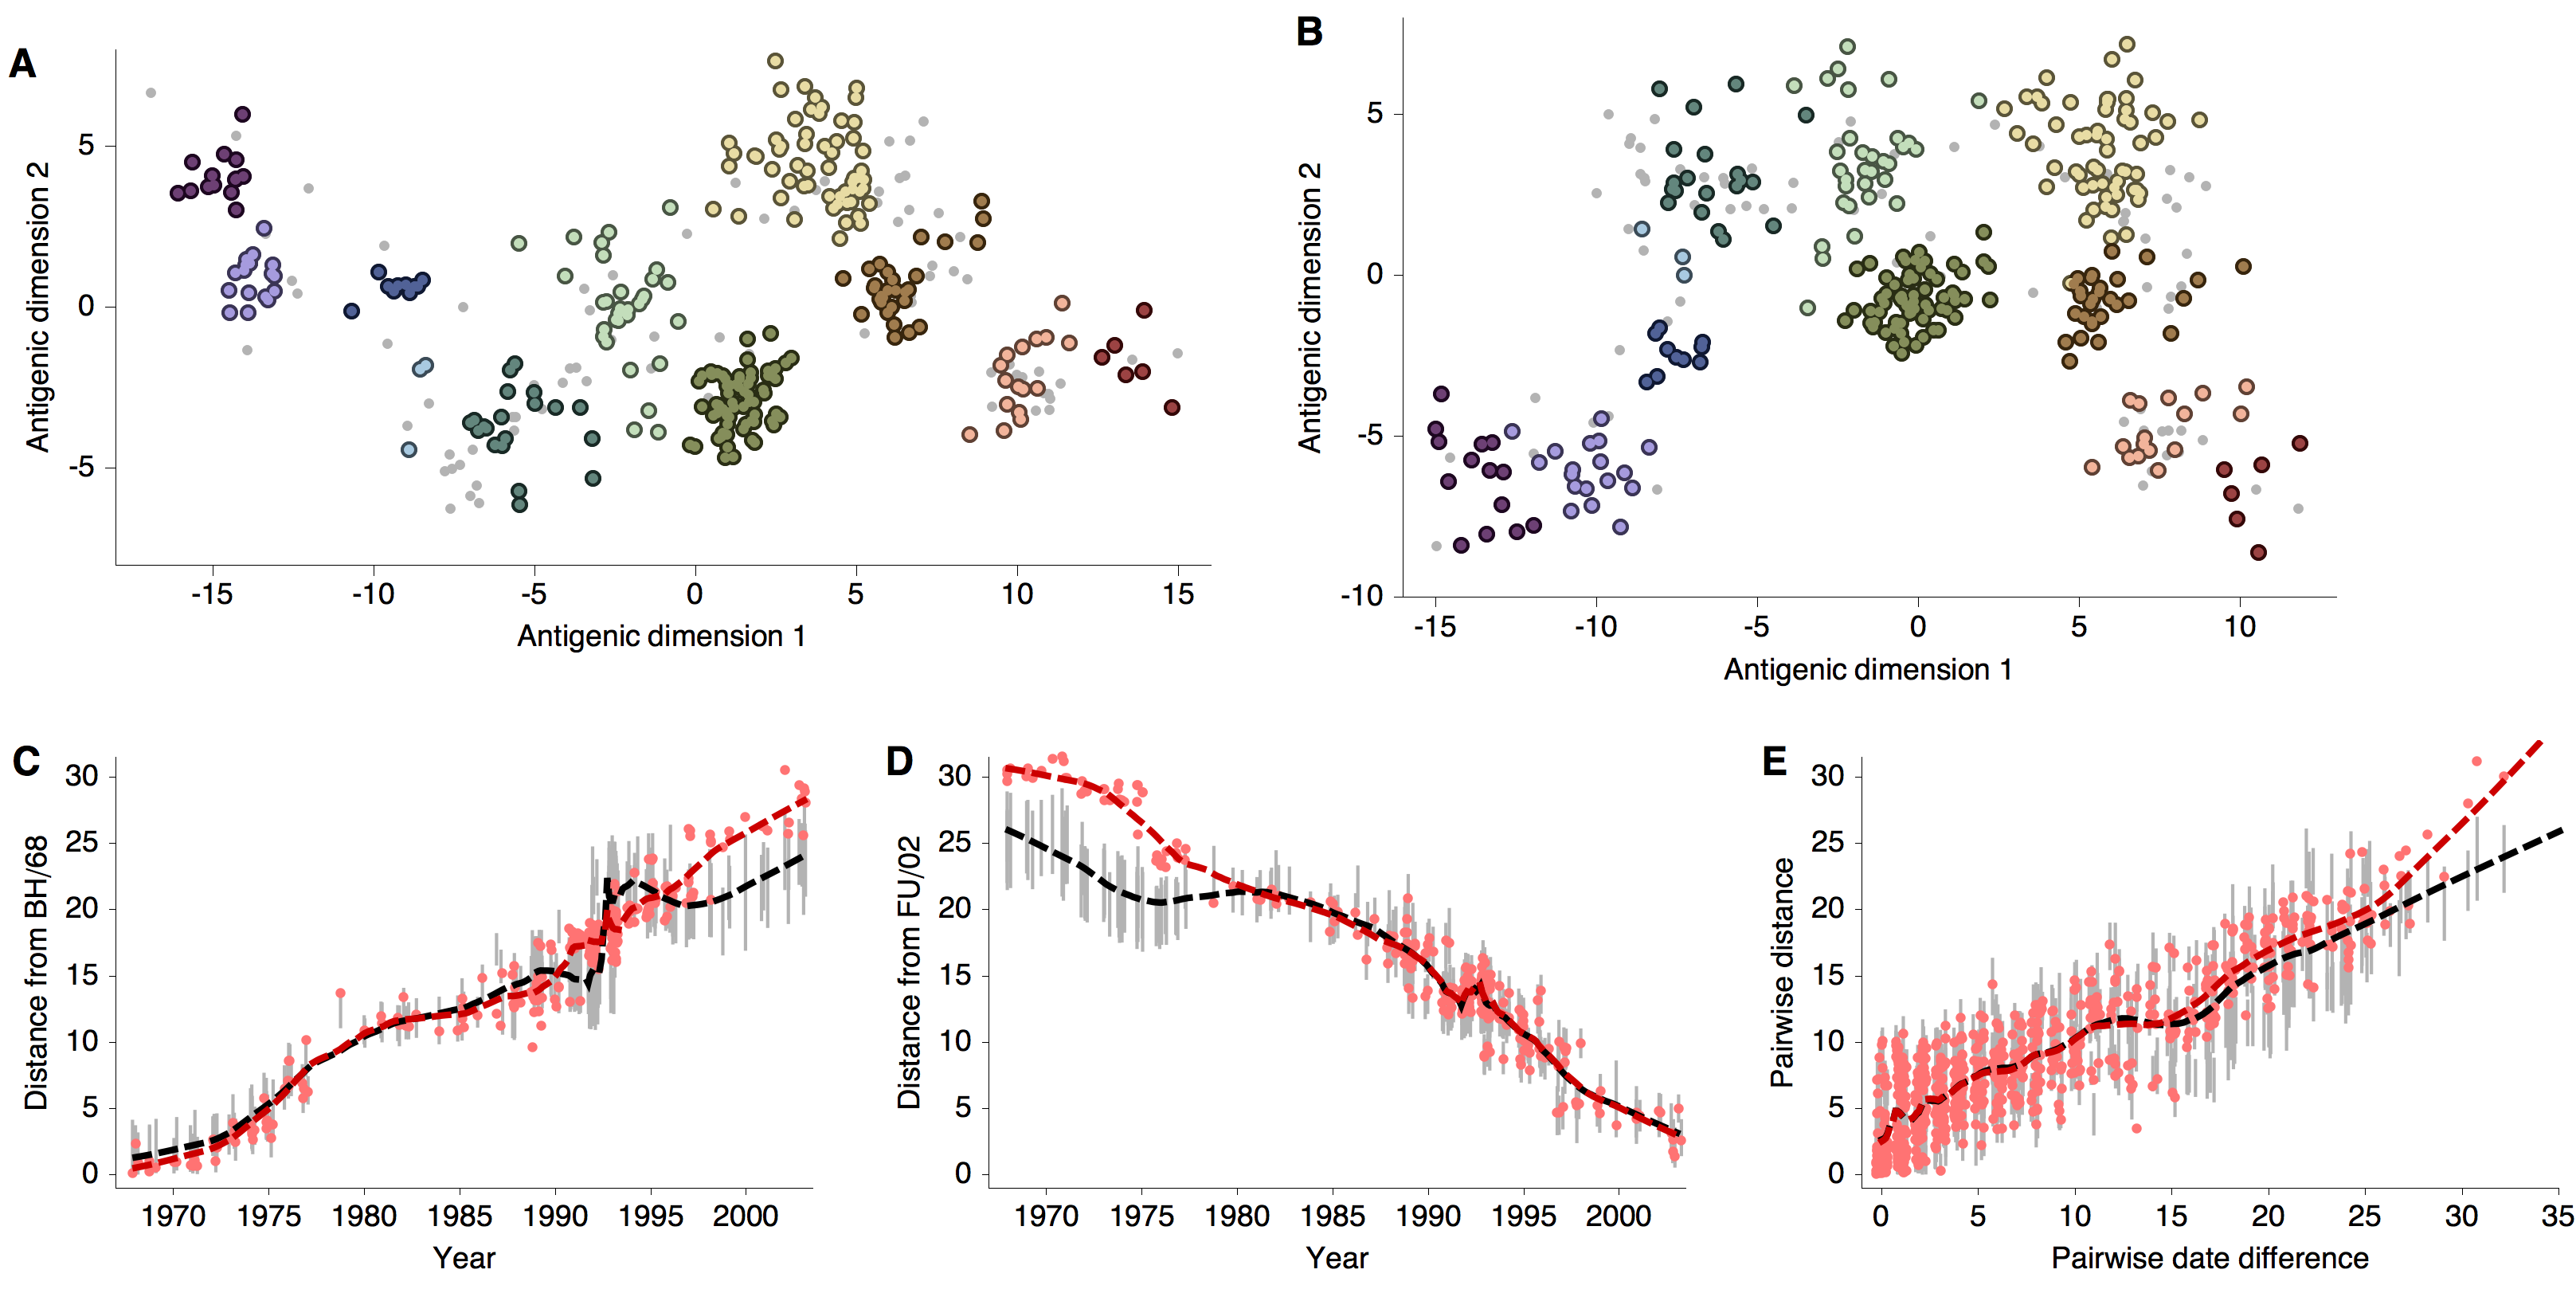
\includegraphics[width=1.0\textwidth]{figures/smith_comparison_rotation}
	\caption{\textbf{Comparison of A/H3N2 antigenic locations estimated by Smith et al.\ \cite{Smith04} using MDS and an equivalent BMDS model under an alternative solution.} 
	(A) MDS antigenic locations, reorientated so that the primary dimension lies on the $x$-axis rather than on the $y$-axis as in Figure 1 of \cite{Smith04}.
	(B) A posterior sample of antigenic locations from an equivalent BMDS model that has converged on the alternative solution.
	In (A) and (B), viruses are shown as colored circles, with color denoting antigenic cluster inferred by \cite{Smith04}, and sera are shown as gray points.
	(C) Antigenic distances between A/Bilthoven/16190/1968 and all other viruses determined for both methods.
	(D) Antigenic distances between A/Fujian/411/2002 and all other viruses determined for both methods.
	(E) Antigenic distances between 750 random pairs of viruses determined for both methods.	
	In (C), (D) and (E) red points show distances for the MDS model and gray bars show the 95\% credible interval of distances for the BMDS model, while the red dashed line shows a LOESS regression to MDS distances, and the black dashed line shows a LOESS regression to the BMDS distances.
	The BMDS model has a Uniform$(-100,100)$ prior on antigenic locations and serum effects fixed at maximum titer values. 	
	} 
	\label{smith_comparison_rotation} 
\end{figure}

As discussed in the main text, the presence of multiple optima with different degrees of 2D curvature implies an issue of identifiability; the HI likelihood model alone cannot distinguish between these possibilities.
Because of this issue, and to more easily estimate rates of antigenic drift, we include a model of systematic drift in antigenic location (discussed in Methods) that favors linear movement in the antigenic map.
We find that including this drift prior on antigenic locations removes the problem of identifiability.
Antigenic locations produced by this model remain locally consistent with MDS results between viruses $\sim$15 years divergent, but global comparisons show that this BMDS model has partitioned more variance to the first antigenic dimension (Figure~\ref{smith_comparison_drift}).
We additionally find that including the drift prior on antigenic locations often results in greater predictive power, with a slight improvement of test error for the A/H1N1, B/Vic and B/Yam datasets (Table~1).

%%% smith_comparison_drift %%%
\begin{figure}[H]
	\centering		
	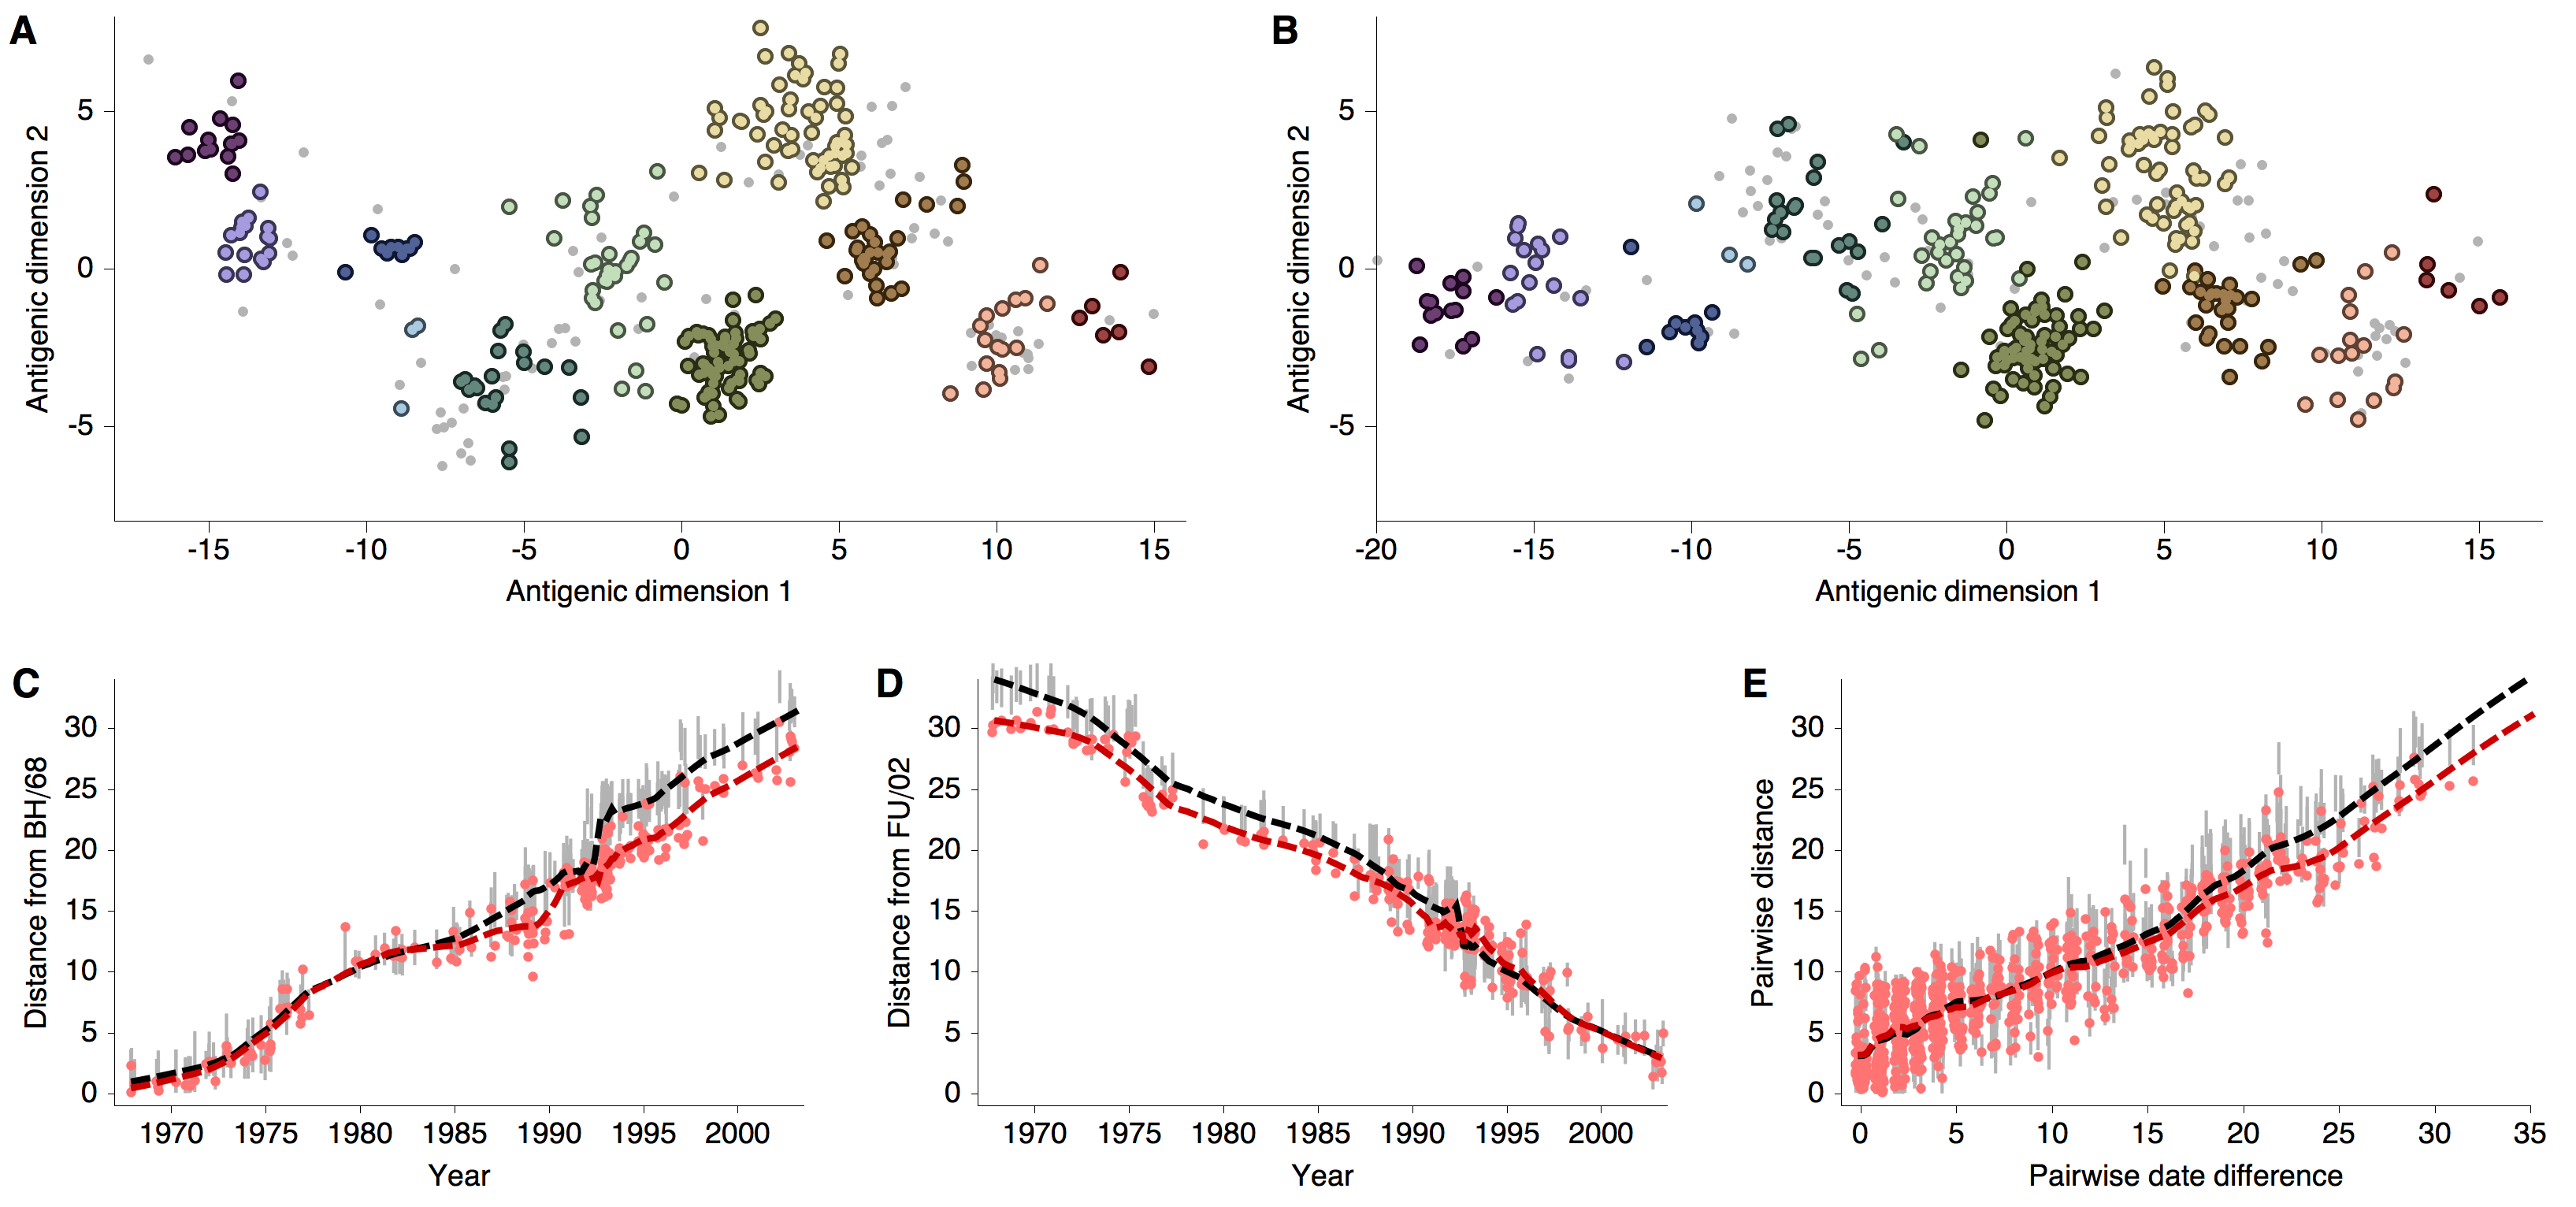
\includegraphics[width=1.0\textwidth]{figures/smith_comparison_drift}
	\caption{\textbf{Comparison of A/H3N2 antigenic locations estimated by Smith et al.\ \cite{Smith04} using MDS and an extended BMDS model that includes date-informed priors on antigenic locations.} 
	(A) MDS antigenic locations, reorientated so that the primary dimension lies on the $x$-axis rather than on the $y$-axis as in Figure 1 of \cite{Smith04}.
	(B) A posterior sample of antigenic locations from a BMDS model that includes date-informed priors on antigenic locations.
	In (A) and (B), viruses are shown as colored circles, with color denoting antigenic cluster inferred by \cite{Smith04}, and sera are shown as gray points.
	(C) Antigenic distances between A/Bilthoven/16190/1968 and all other viruses determined for both methods.
	(D) Antigenic distances between A/Fujian/411/2002 and all other viruses determined for both methods.
	(E) Antigenic distances between 750 random pairs of viruses determined for both methods.	
	In (C), (D) and (E) red points show distances for the MDS model and gray bars show the 95\% credible interval of distances for the BMDS model, while the red dashed line shows a LOESS regression to MDS distances, and the black dashed line shows a LOESS regression to the BMDS distances.
	The BMDS model has a date-informed prior on antigenic locations and serum effects fixed at maximum titer values. 	
	} 
	\label{smith_comparison_drift} 
\end{figure}

Our final BMDS model (model 9, Table 1) differs from antigenic model used by Smith et al.\ \cite{Smith04} in including temporally- and phylogenetically-informed priors on antigenic locations and also in estimating serum and virus effects (discussed in Methods).
Here, we investigate the impact on antigenic locations of estimating virus and serum effects in the BMDS model.
To isolate this difference, we use a Uniform$(-100,100)$ prior on antigenic locations.
Surprisingly, estimating virus and serum effects results in a more linear antigenic map (Figure~\ref{smith_comparison_effects}), resembling the appearance of the map incorporating the antigenic drift prior, while preserving local consistency.
We generally observe congruence between MDS and BMDS antigenic locations for viruses less than $\sim$10 years divergent (Figure~\ref{smith_comparison_effects}E).
However, specific viruses may be affected, for instance A/Bilthoven/16190/1968 (Figure~\ref{smith_comparison_effects}C), which appears more distant from all other viruses when serum and virus effects are included.

%%% smith_comparison_effects %%%
\begin{figure}[H]
	\centering		
	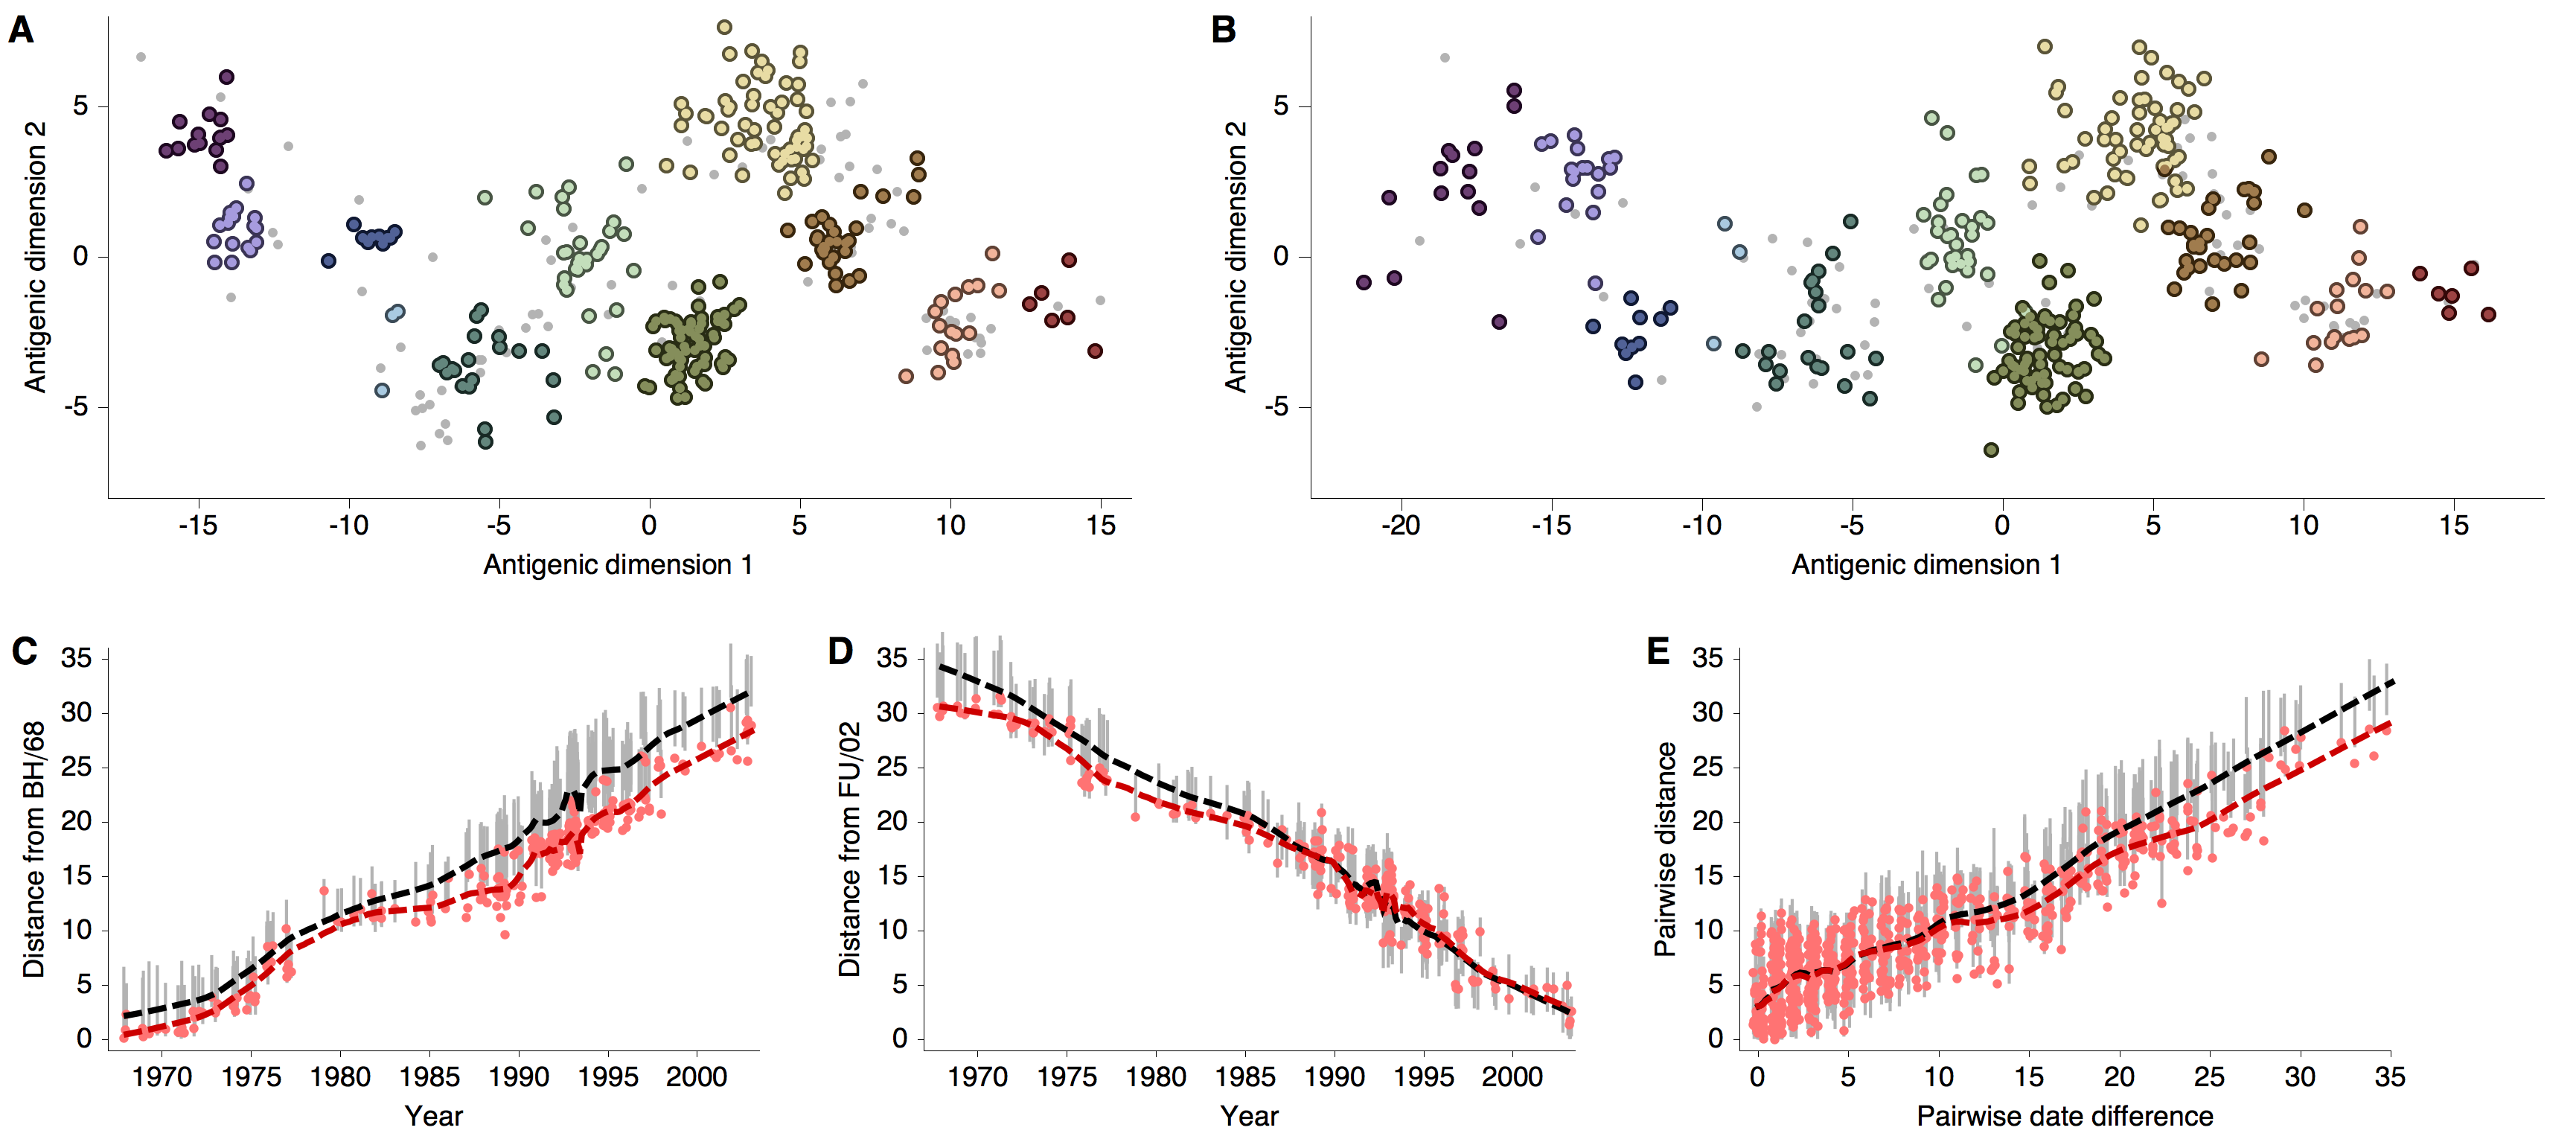
\includegraphics[width=1.0\textwidth]{figures/smith_comparison_effects}
	\caption{\textbf{Comparison of A/H3N2 antigenic locations estimated by Smith et al.\ \cite{Smith04} using MDS and an extended BMDS model that estimates serum and virus effects.} 
	(A) MDS antigenic locations, reorientated so that the primary dimension lies on the $x$-axis rather than on the $y$-axis as in Figure 1 of \cite{Smith04}.
	(B) A posterior sample of antigenic locations from a BMDS model that estimates virus and serum effects.
	In (A) and (B), viruses are shown as colored circles, with color denoting antigenic cluster inferred by \cite{Smith04}, and sera are shown as gray points.
	(C) Antigenic distances between A/Bilthoven/16190/1968 and all other viruses determined for both methods.
	(D) Antigenic distances between A/Fujian/411/2002 and all other viruses determined for both methods.
	(E) Antigenic distances between 750 random pairs of viruses determined for both methods.	
	In (C), (D) and (E) red points show distances for the MDS model and gray bars show the 95\% credible interval of distances for the BMDS model, while the red dashed line shows a LOESS regression to MDS distances, and the black dashed line shows a LOESS regression to the BMDS distances.
	The BMDS model has a Uniform$(-100,100)$ prior on antigenic locations and virus and serum effects estimated in a hierarchical Bayesian fashion. 	
	} 
	\label{smith_comparison_effects} 
\end{figure}

In this dataset, viruses 15 or more years divergent always yield threshold titers, and hence, their relative locations must be indirectly inferred rather than through direct comparison.
This may explain why we observe local consistency between models at scales less than $\sim$15 years, but some degree of global inconsistency.
Still, these results suggest that, when making local comparisons, such as those used to calculcate year-to-year antigenic drift (Figure 3), outcomes are expected to be robust to  many model particulars.

%%% REFERENCES %%%
\bibliographystyle{plos}
\bibliography{flux}

\end{document}